% !TEX root=../../mt-motion-analysis.tex
\chapter{Related work - Time Series Classification} \label{sec:tsc} \label{ch:tsc}
\section{Background - Time series classification}
Time series are sequences of data ordered in some dimension, e.g. time. They can be univariate, i.e. containing one variable, or multivariate and they can be used to describe any ordered, discrete data, for instance information extracted from videos.

\begin{definition}
  \text{A univariate time series of length n, with ordered indices}
  $$X = \left[x_1, x_2, \hdots, x_n\right]^\intercal$$
  \label{def:uts}
\end{definition}

\begin{definition}
    \text{A multivariate time series of length n, with M channels}
    $$\pmb{X} = \left[X_1, \hdots, X_M\right]$$
\end{definition}

The \gls{tsc} task is about finding a function, $f: \mathbb{R}^{n \times M} \rightarrow \mathbb{R}$, that assigns one label to each, possibly multivariate, time series. The problem bears strong resemblance with that of image classification, but with the two spatial dimensions replaced by one temporal dimension. Despite this the use of end-to-end deep learning models is not as dominant in the \gls{tsc} community \cite{IsmailFawaz2019}. Instead it is common to manually extract features deemed suitable for classification. Similarily to the fields of computer vision various datasets has emerged recently. This has been important for the development of \gls{tsc} as it allows for fair comparison between methods. One of the most widely used dataset collections today is the \gls{ucr} archive \cite{Dau2018} containing 85 different time series datasets.

Traditionally a nearest neighbor method together with dynamic time warping has been common for classification \cite{Bagnall2017}. Simply put, this means that a time series during classification is compared to the training data and assigned the class of the most similar time series. Lines and Bagnall suggested a method where an ensemble of 11 nearest neighbor classifiers with different similarity measures \cite{Lines2015} which yielded \gls{sota} results. Bagnall et al. \cite{Bagnall2015} developed the idea of ensemble based classifiers with \gls{cote}, where 35 different classifiers using different transforms were used.
Lines et al. \cite{Lines2016} extended \gls{cote} further with two new classifiers resulting in \gls{hive-cote}. One drawback with \gls{hive-cote} is the computational intensity, both during training and test time. Training time is large partly due to one of the transforms used is the Shapelet Transform with a time complexity of $O(n^2l^4)$, $n$ being the number of time series and $l$ the length of them. Due to the nature of the nearest neighbor algorithm, the result of the 37 classifiers during test time needs to be compared to the corresponding result for each time series in the training set, causing this method to be impractical for real-time use \cite{IsmailFawaz2019}.

In 2016 Zheng et al. \cite{Zheng2016} presented a neural network model based on convolutional layers for the classification task. Wang et al. \cite{Wang2017} developed these ideas and presented models with performance close to that of \gls{cote} on the \gls{ucr} archive. The development of neural network based classification has since then continued and below two architectures which are either used or have inspired our work are presented.

\section{Deep learning architectures}
The last few years the number of proposed neural network based time series classifiers has increased drastically. Below the two most influential architectures for our work are presented.

\subsection{InceptionTime} \label{sec:inception-time}
InceptionTime, presented by Fawaz et al. \cite{IsmailFawaz2020}, is, as the name suggests, inspired by Inception \cite{Szegedy2015} which is an architecture successful in computer vision tasks. It is comprised of several stacked Inception modules consisting of differently sized convolutions as well as pooling layers. To reduce the number of parameters in the network 1$\times$1 convolutions are often used as a dimensionality reduction.
One such module can be seen in Figure \ref{fig:inception-module}. The architecture of Fawaz et al. is similar, but with only one temporal dimension instead of two spatial dimensions. The number of filters in the convolutions and the length of these filters are hyperparameters to be tuned. All convolutions use the same number of filters to simplify the tuning and the same length parameter is also used throughout the network. The length of the three parallel filters is given by $0.5^k* \text{filter\_length}$, $k = [0,1,2]$. Thus the length parameter in Figure \ref{fig:inception-module} is 40. As with the computer vision task the dimensionality is reduced, here through a bottleneck of size $m$. The bottleneck is achieved by convolutions with $m$ filters of length 1. The InceptionTime module is shown in Figure \ref{fig:inceptiontime-module}.

Figure \ref{fig:inceptiontime} shows how stacked modules makes up the InceptionTime architecture. Residual connections are used to decrease the risk of vanishing gradients once the network becomes deeper, as suggested by He et al. \cite{He2016}. The InceptionTime modules are followed by a \gls{gap} layer which averages each time series over its time dimension. The classification is performed by fully connected layers with softmax activations.

Many deep learning based time series classifiers experiences a significant variance in their accuracy, especially when evaluated on the \gls{ucr} archive with rather small training sets \cite{IsmailFawaz2019ensemble}. To overcome this Fawaz et al. suggest the use of an ensemble of identical InceptionTime networks, but with randomly initialized weights before training. The ensemble's output is then calculated as the average of the outputs of the individual models. Such an ensemble of five models achieves a performance similar to that of \gls{hive-cote} on the \gls{ucr} archive.
% As was showed with ResNet \cite{He2016} residual connections reduces the risk for vanishing gradients and enables deeper networks. Hence this is

% Using residual connections between blocks reduces the risk of vanishing gradients and allows for deeper networks

%The 1D convolutions together with dimensionality reduction allows for longer filters than what is feasible to use for images.

\begin{figure}
  \centering
  \begin{subfigure}[c]{0.6\textwidth}
    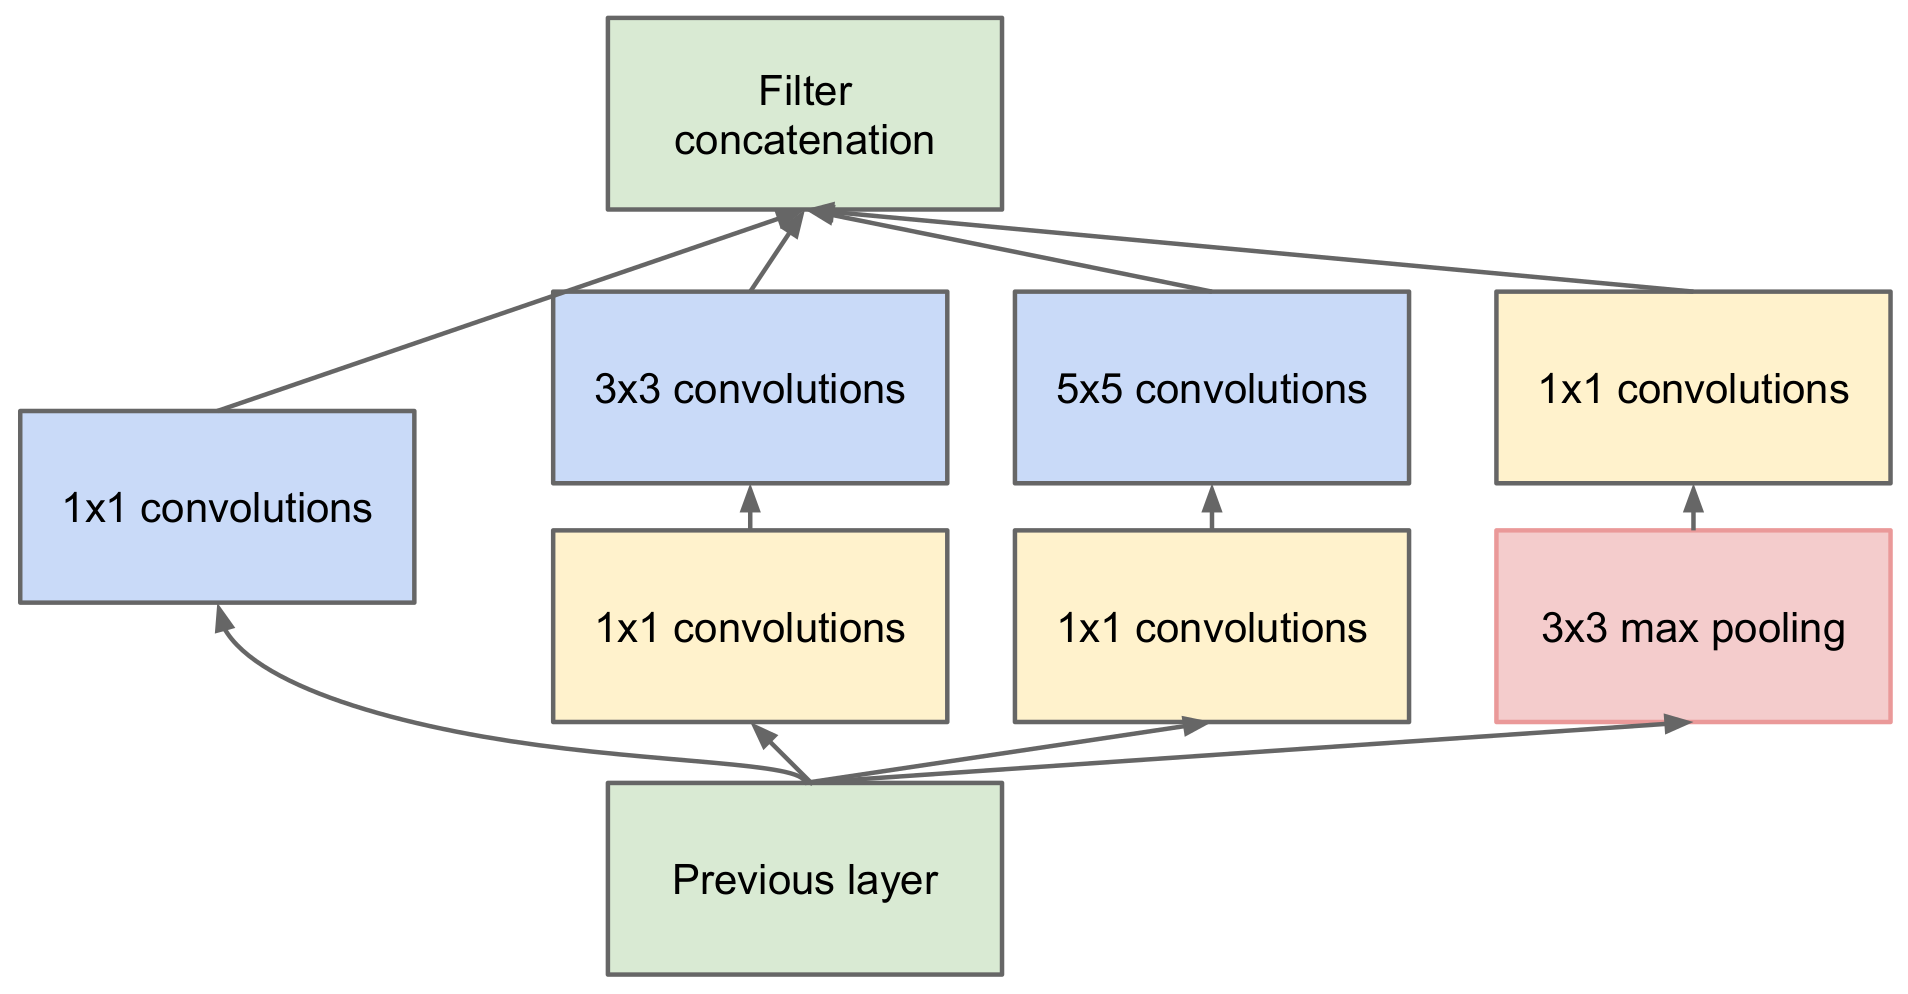
\includegraphics[width=\textwidth]{files/figs/tsc/inception-module-dimred.png}
    \caption{}
    % \caption{Inception module for computer vision \cite{Szegedy2015}.}
    \label{fig:inception-module}
  \end{subfigure}
  \begin{subfigure}[c]{0.6\textwidth}
    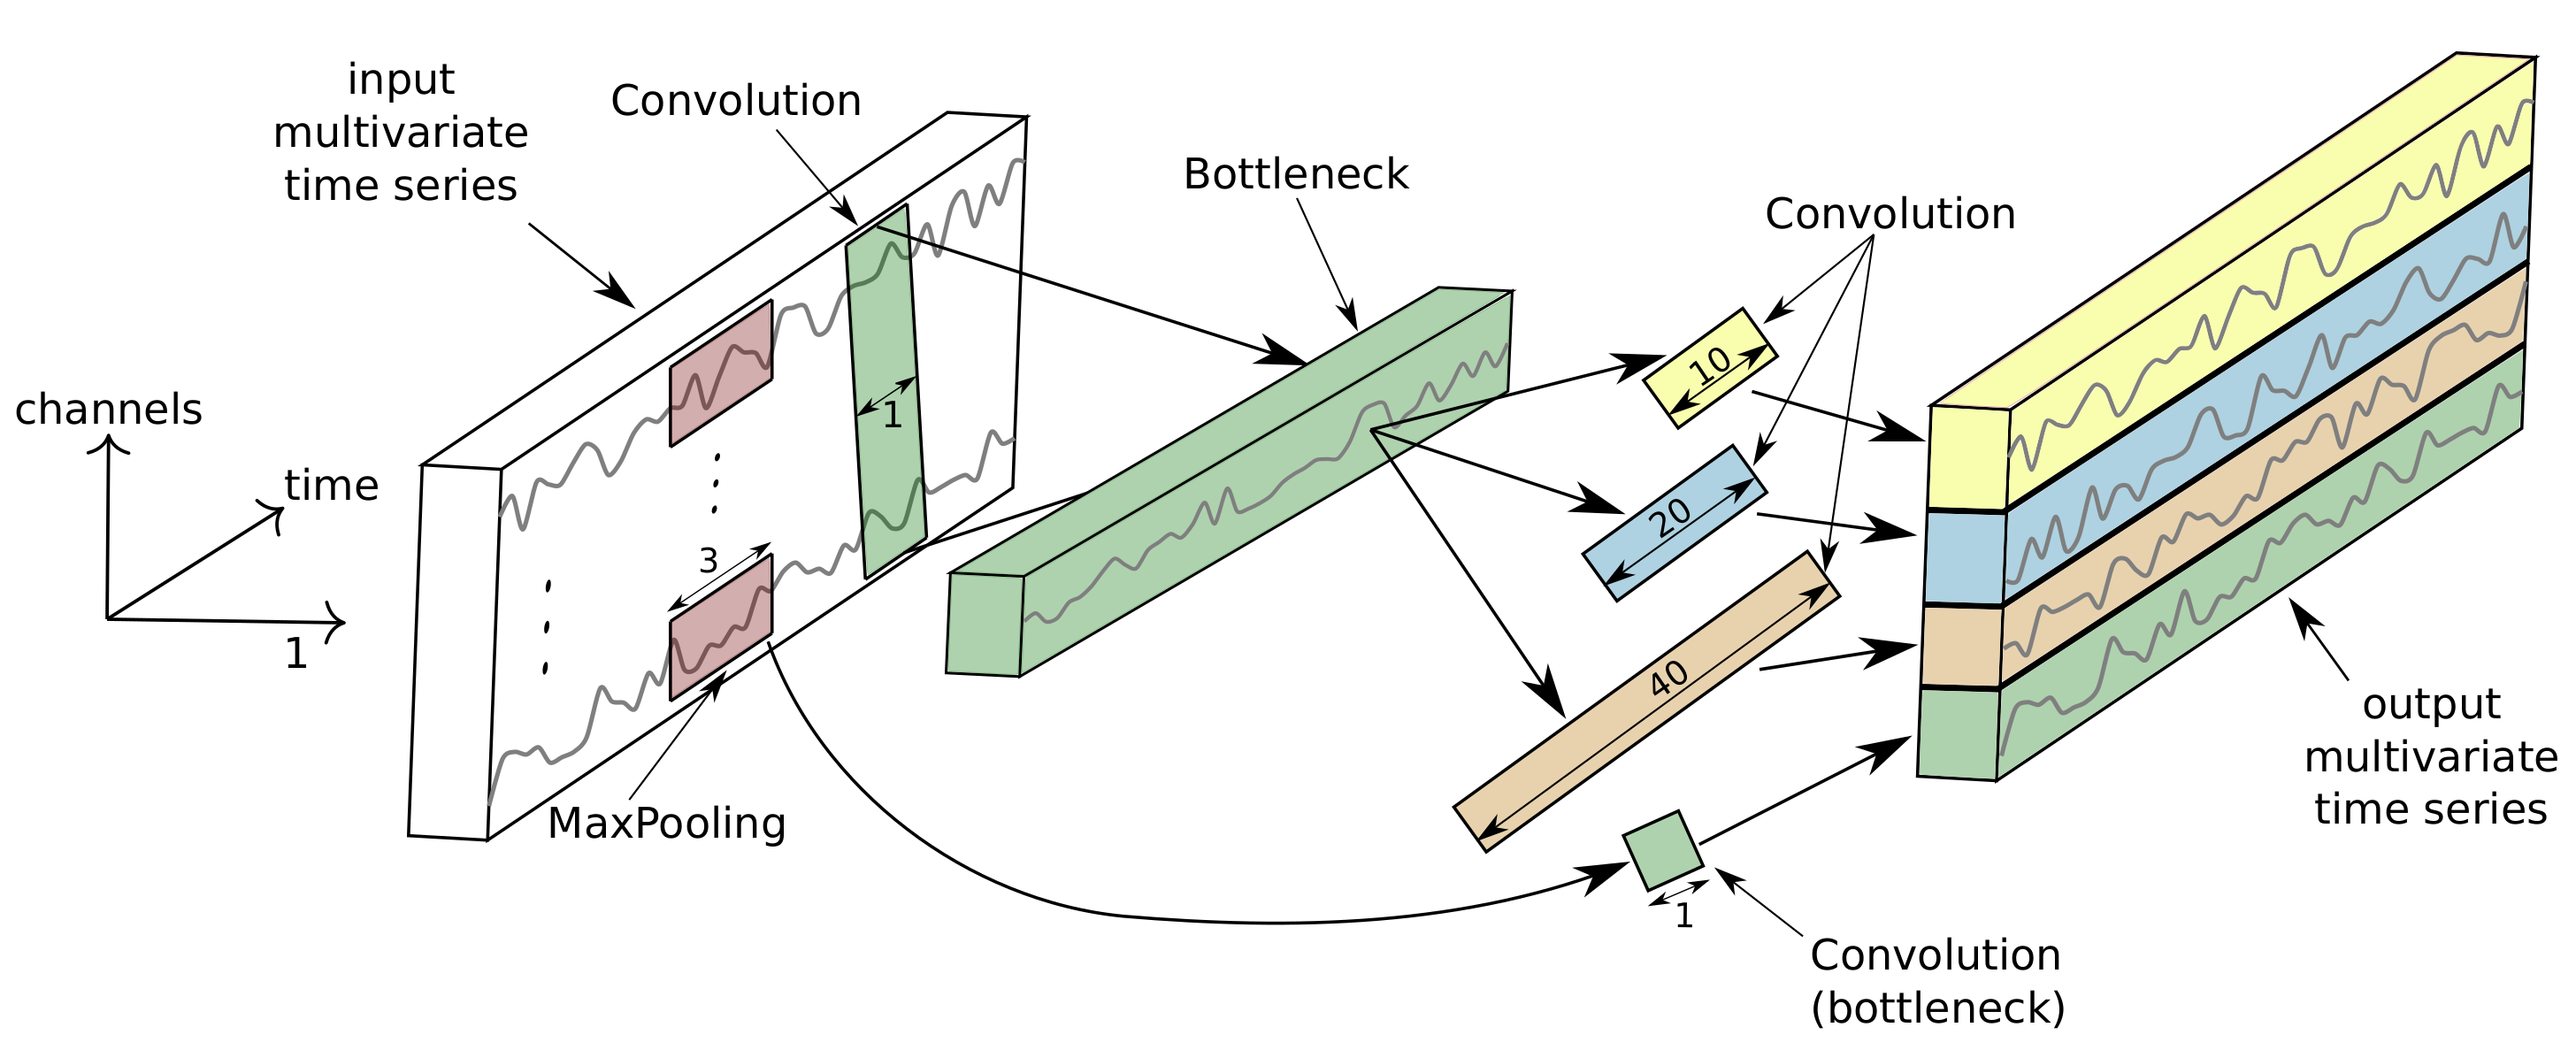
\includegraphics[width=\textwidth]{files/figs/tsc/inception-time-module.png}
    \caption{}
    % \caption{Inception module for \gls{tsc} \cite{IsmailFawaz2020}.}
    \label{fig:inceptiontime-module}
  \end{subfigure}
  \caption{Inception modules for computer vision (a) with dimensionality reduction ahead of the 3$\times$3 and 5$\times$5 convolutions and InceptionTime module for TSC (b), here illustrated with a bottleneck size of 1. Figures from \cite{Szegedy2015} and \cite{IsmailFawaz2020} respectively.}
\end{figure}

\begin{figure}
  \centering
  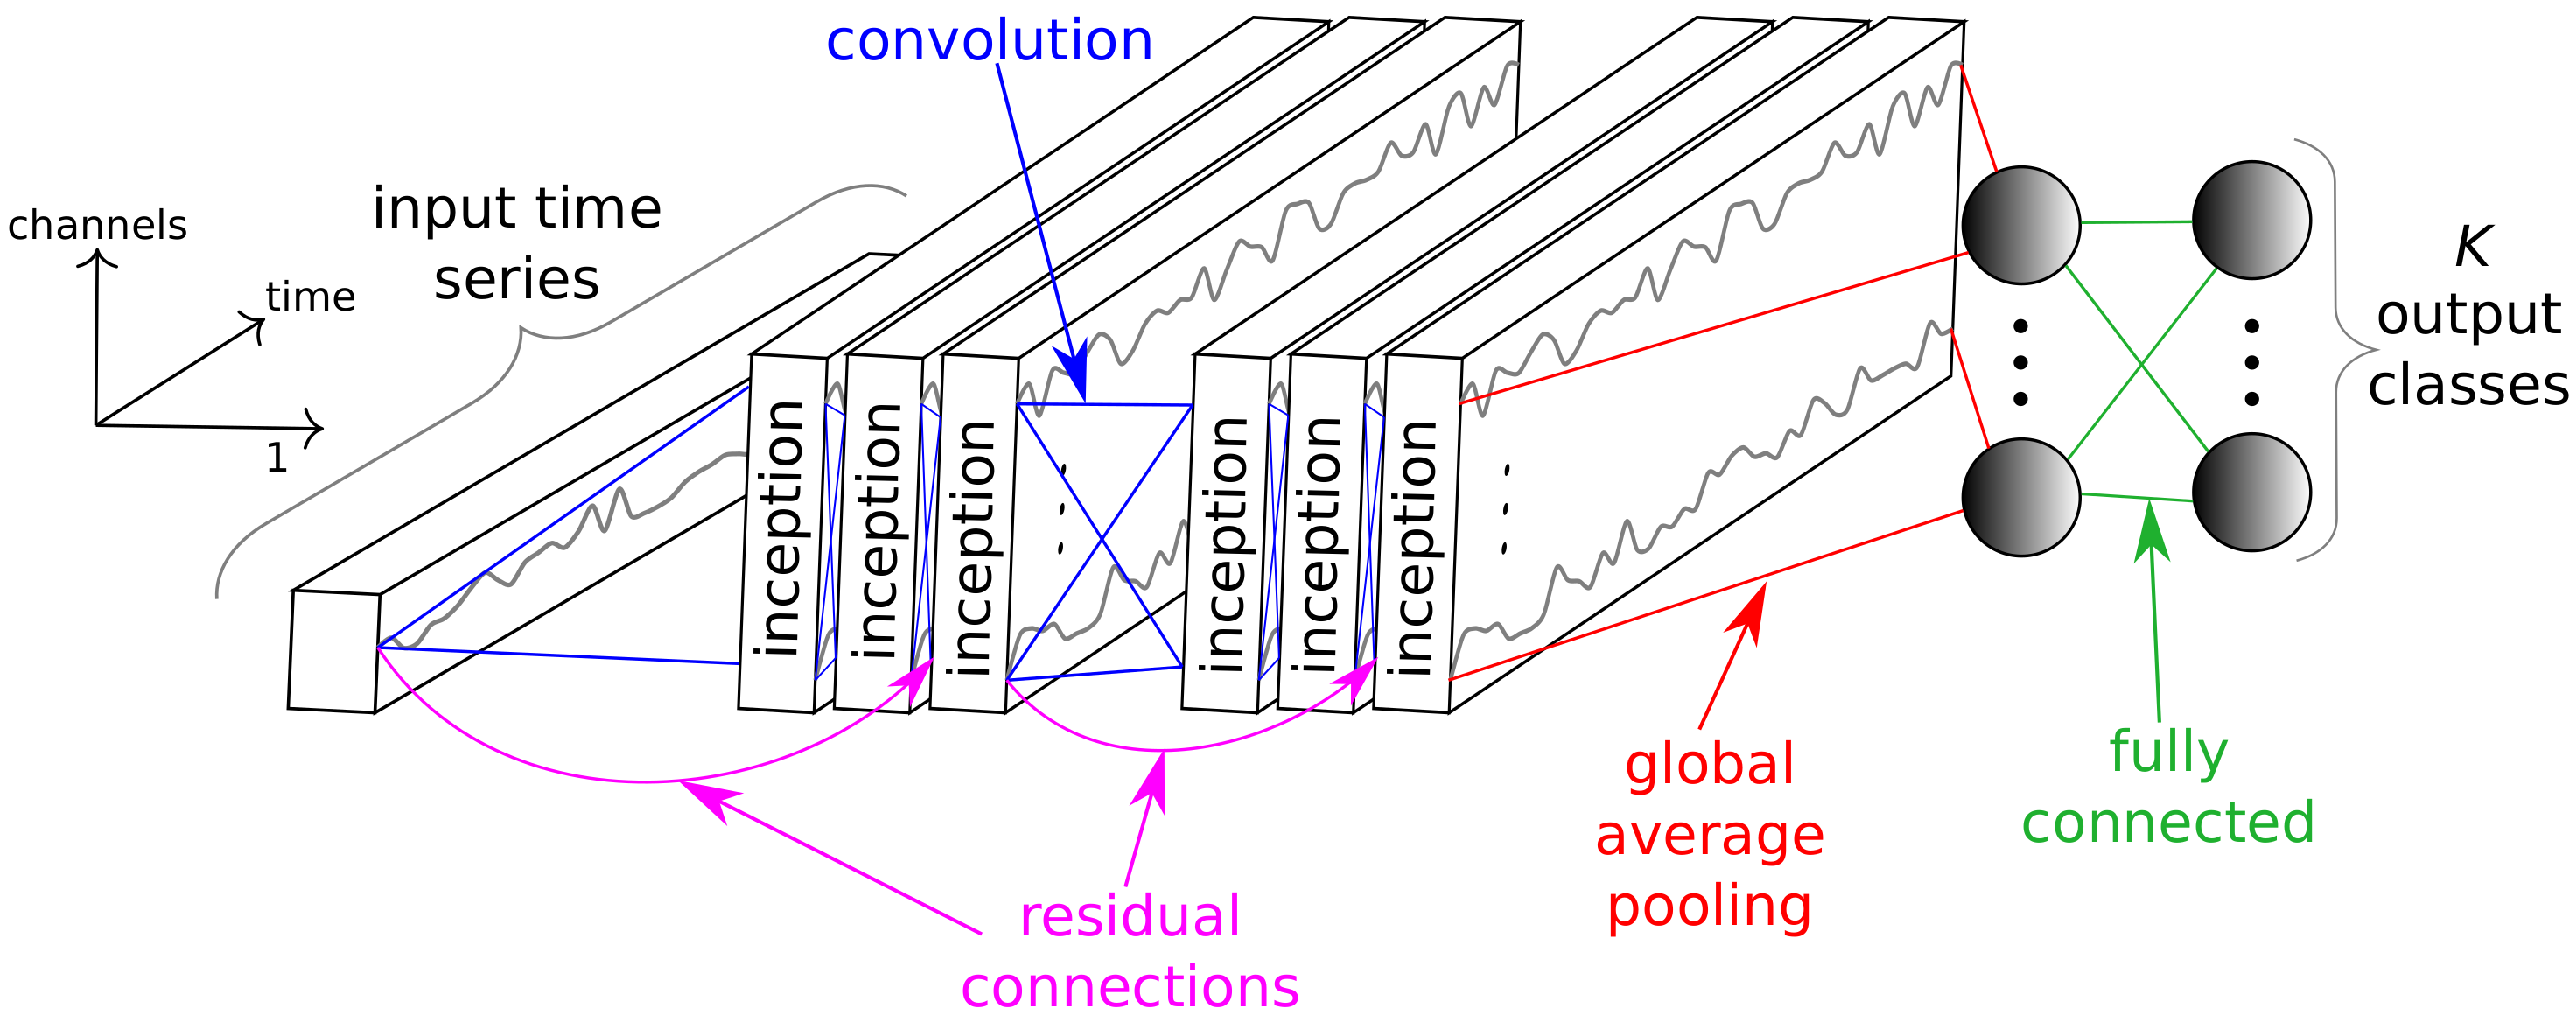
\includegraphics[width=0.6\textwidth]{files/figs/tsc/inceptiontime.png}
  \caption{InceptionTime architecture for TSC \cite{IsmailFawaz2020}.}
  \label{fig:inceptiontime}
\end{figure}

% \FloatBarrier

\subsection{Explainable Convolutional Neural Network for Multivariate Time Series Classification (XCM)} \label{sec:XCM}
As discussed in Section \ref{sec:explainability} explainability is desirable, but not inherent in most black-box deep learning models. Fauvel et al. \cite{Fauvel2020} propose an architecture, \gls{xcm}, which allows for tracking which time steps and which inputs are important for the classification decision. By using 2D convolutions with kernels of size $ks$$\times$1, where $ks$ is the kernel size hyperparameter, the convolution is only performed in the time dimension and the input channels are kept separated throughout the feature extraction.
Through dimensionality reduction from a 1$\times$1 2D convolution a single feature map for each input is produced. From this, the importance of input channels and time steps can be traced using \gls{grad-cam}, described in Section \ref{sec:grad-cam}. In parallel to the channel specific features Fauvel et al. also suggests using 1D convolutions over all channels resulting in a combined feature map along the time dimension. The \gls{xcm} architecture is depicted in Figure \ref{fig:xcm}.

\begin{figure}
  \centering
  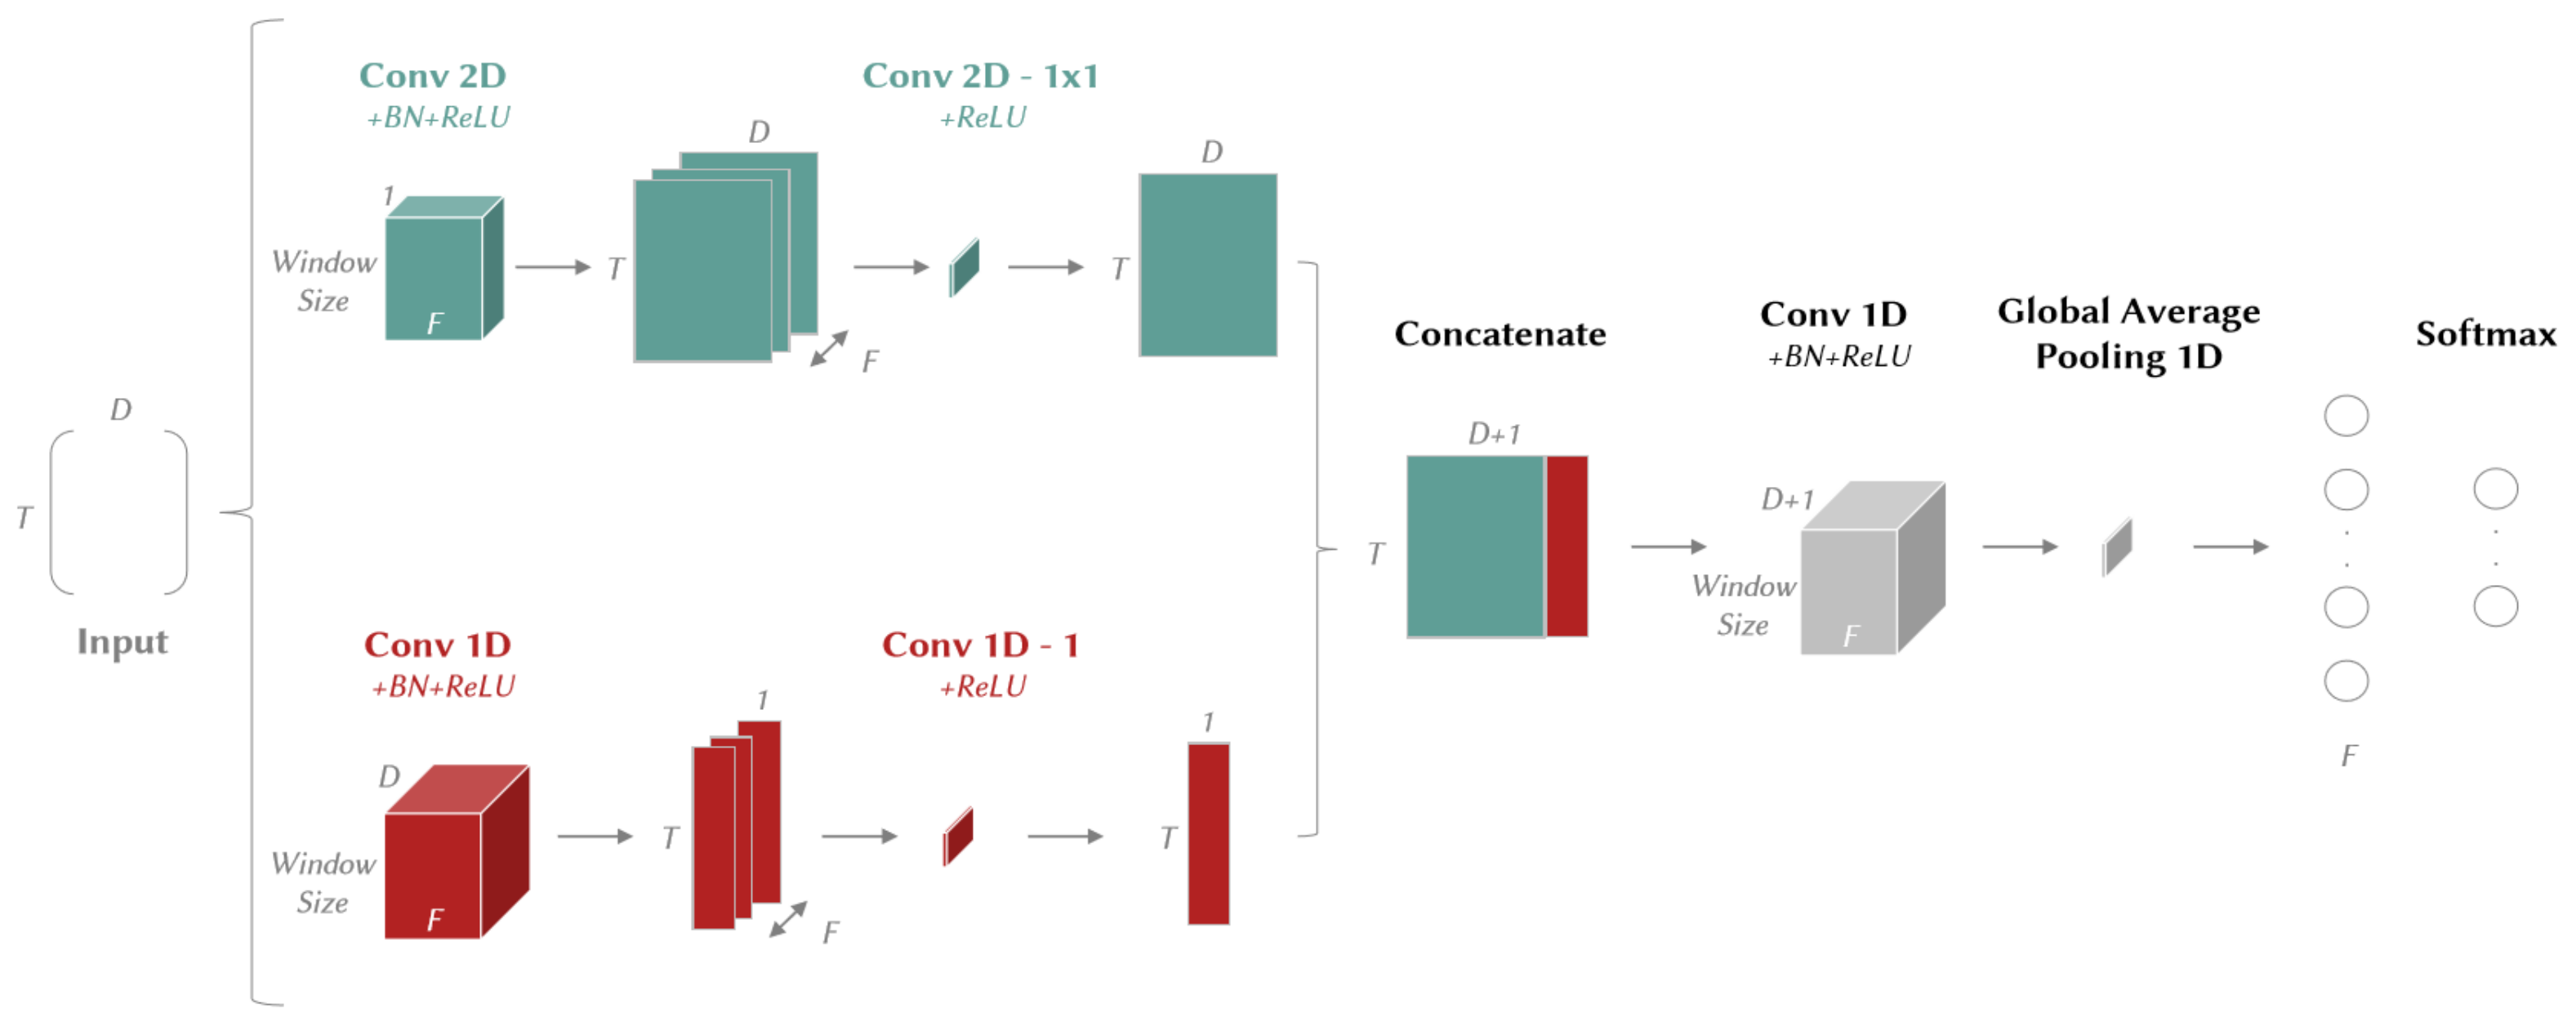
\includegraphics[width=0.7\textwidth]{files/figs/tsc/xcm.png}
  \caption{The XCM architecture with $BN$ - Batch Normalization, $D$ - number of input channels, $F$ - number of filters, $T$ - length of time series \cite{Fauvel2020}.}
  \label{fig:xcm}
\end{figure}

% \FloatBarrier
